\chapter{Trabalhos Relacionados}
\label{c_estado_arte}

Este capítulo apresenta trabalhos similares ao que se propõe nesta pesquisa. Ele está dividido em três seções. A \autoref{sec_tools} apresenta ferramentas que buscam auxiliar crianças nos primeiros contatos com algoritmos por meio da depuração. A \autoref{sec_rsl} apresenta uma revisão sistemática da literatura (RSL) sobre pesquisas que observam a interação de crianças de 3 a 6 anos com BPs. A intenção é compreender quais interfaces são comumente utilizadas, quais são os designs experimentais aplicados e que resultados são obtidos, para fundamentar a escolha do design experimental desta pesquisa. Por fim, a \autoref{secao_mapeamento_industrial} apresenta um mapeamento industrial\footnote{Método de busca baseado em fontes não acadêmicas, mas que segue um método sistemático. Também chamado de mapeamento industrial sistemático.} sobre as interfaces de BPs, que demonstra quais tipos de interface estão disponíveis no comércio eletrônico. %Enquanto na \autoref{sub_sub_aplicacoes_ra_projetiva_educacao} apresenta aplicação de RA projetiva em ferramentas educacionais, o mapeamento indica que a técnica   no contexto de BPs.

\section{Interfaces de Brinquedos Programáveis}
\label{sec_tools}
Esta seção tem por objetivo demonstrar interfaces para crianças terem os primeiros contatos com algoritmos utilizando BPs. Para isso, identifica as características de cada trabalho e compara com a solução proposta. Os critérios utilizados para a escolha dos trabalhos relacionados foram o público-alvo (crianças a partir dos 4 anos), a visibilidade dos algoritmos por meio de interfaces tangíveis e o uso de BPs. Assim, foram analisados quatro trabalhos:

\begin{enumerate}
    \item Robo-Blocks: uma interface tangível eletrônica para programação de BPs, com foco em ensino de depuração \cite{sipitakiat_robo-blocks_2012}.
    \item Cubetto: um BP com interface tangível de painel, que indica a execução de cada comando por meio de luzes (\url{https://www.primotoys.com}).
    \item Bee-Bot com mesa interativa: uma mesa interativa com objetos tangíveis, que projeta um mapa interativo que reage aos posicionamento dos objetos físicos em sua superfície \cite{beraza_soft_2010}.
    \item ALERT: interface de programação interativa, na qual o BP interpreta comandos à medida que os detecta via câmera \cite{burleson_active_2018}.
\end{enumerate}

\subsection{Robo-Blocks}
O Robo-Blocks, de \citeonline{sipitakiat_robo-blocks_2012}, é um sistema que permite que crianças comandem um BP por meio do encaixe de blocos eletrônicos. Os quatro movimentos básicos do robô são iguais aos do brinquedo RoPE (mover-se para frente, para trás, girar à esquerda e girar à direita), porém as crianças também podem parametrizar a extensão do movimento do robô ajustando um controle giratório presente em cada bloco (\autoref{fig:robo_blocks}). Os blocos são encaixados por conectores magnéticos, formando uma sequência. Essa sequência se liga a um bloco principal, que envia os comandos ao BP por comunicação sem fio. O BP, por sua vez, é inspirado na tartaruga do ambiente Logo. Ele tem uma caneta acoplada que permite desenhar ao serem utilizados blocos de \textit{"pen up"} (erguer caneta) e \textit{"pen down"} (baixar caneta).

\begin{figure}[!h]
    \centering
    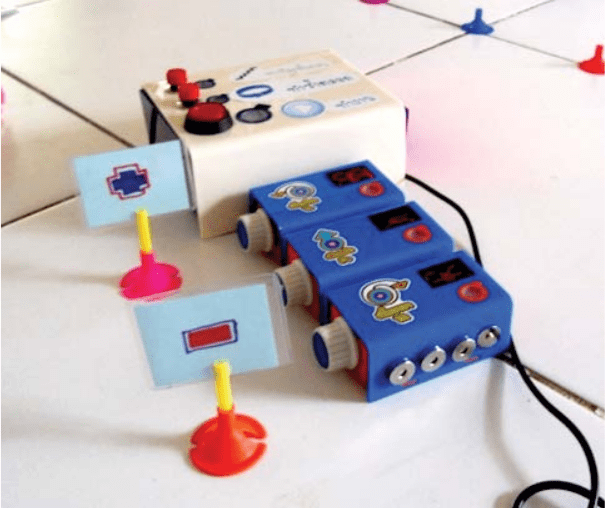
\includegraphics[width=.7\linewidth,fbox]{figs/robo_blocks.png}
    \caption{Robo-Blocks.}
    \label{fig:robo_blocks}
\end{figure}
O Robo-Blocks foi inicialmente desenvolvido com uma interface tangível sem atenção ao processo de depuração. Entretanto, os pesquisadores perceberam que as crianças costumavam direcionar sua atenção para os movimentos do robô, sem prestar atenção nos blocos, o que dificultava encontrar erros. Para resolver este problema os autores criaram a função de execução passo a passo, que permite gerenciar a execução e encontrar erros com mais facilidade.

Além da execução passo a passo, os autores utilizam "objetos passivos", ou seja, que não influenciam na execução do robô. No caso foi utilizado pequenas bandeiras com as quais a criança identifica os blocos que podem ser a causa de erros. As bandeiras têm ícones de "mais" e "menos". Deste modo, a criança pode colocar a bandeira com sinal positivo ao lado do bloco para indicar que o robô deve girar mais ou mover-se mais para frente, por exemplo.

Outro objeto utilizado para auxiliar na depuração foi o protractor. Destinado a solucionar dúvidas com relação à ângulos, é um simples pedaço de papel com um furo no centro, por onde o robô passa. Quando o robô está parado, a criança coloca o protractor na mesa, sobre o robô. Ao redor do furo há marcações de ângulos, de modo que a criança consegue estimar o quanto o robô precisa se mover relativo à sua direção atual.

Testes com o Robo-Blocks ocorreram com crianças de 5 a 12 anos, porém o estudo formal focou em crianças de 8 a 9. Esse estudo consistiu em atividades de programar o robô para desenhar a primeira letra do nome e andar em um mapa. Os autores identificaram que as crianças tiveram dificuldades em concluir as atividades e recorreram às funções de depuração. Um problema estava no fato de a criança não conseguir observar a cadeia de comandos e robô simultaneamente. Neste sentido, a execução passo a passo foi o modo preferido pelas crianças. O uso das bandeiras para marcar os erros também foi comum, porém os autores ressaltam que a presença de um erro no início da cadeia de blocos interfere em todos os demais movimentos do robô, de modo que parecem também estar errados. Essa característica levava as crianças a marcar todos os demais blocos como errados. Neste caso, os pesquisadores precisaram intervir corrigindo a posição do robô manualmente.

\subsection{Cubetto}
\label{sub_sec:cubetto}
O Cubetto é um brinquedo programável feito de madeira e destinado a crianças entre 4 a 8 anos, que foi desenvolvido pela empresa PrimoToys\footnote{\url{https://www.primotoys.com}} a partir de 2013. Ele se inspira no ambiente LOGO, pois se move no chão como a tartaruga robótica desenvolvida de Papert. Além disso, o seu design é inspirado no método Montessori, que incentiva o aprendizado autônomo por meio da interação com materiais concretos, lúdicos.

Os algoritmos que definem os movimentos do Cubetto são feitos com blocos coloridos encaixados em um painel. Há 7 tipos de blocos, sendo quatro blocos direcionais e três blocos lógicos. Os blocos direcionais são frente (verde), trás (roxo), giro à esquerda (amarelo) e giro à direita (vermelho). Os blocos lógicos são movimento aleatório (preto), negação (marrom) e função (azul). O bloco de movimento aleatório sorteia um movimento direcional, possibilitando trajetos diferentes com um mesmo algoritmo. O bloco de negação é associado a um bloco de movimento, modificando-o para movimento contrário. Por exemplo, se o próximo bloco é girar para a esquerda, então o brinquedo gira para a direita. Por fim, o bloco de função faz com que os blocos encaixados em uma área inferior do painel (área de função) sejam executados. Esses blocos especiais, portanto, permitem estender o comportamento além de sequências de comandos. Um bloco de função posicionado na área de função, por exemplo, cria uma função recursiva. Se esta função tiver um bloco de movimento aleatório, o brinquedo executará movimentos diferentes indefinidamente.

\begin{figure}
    \centering
    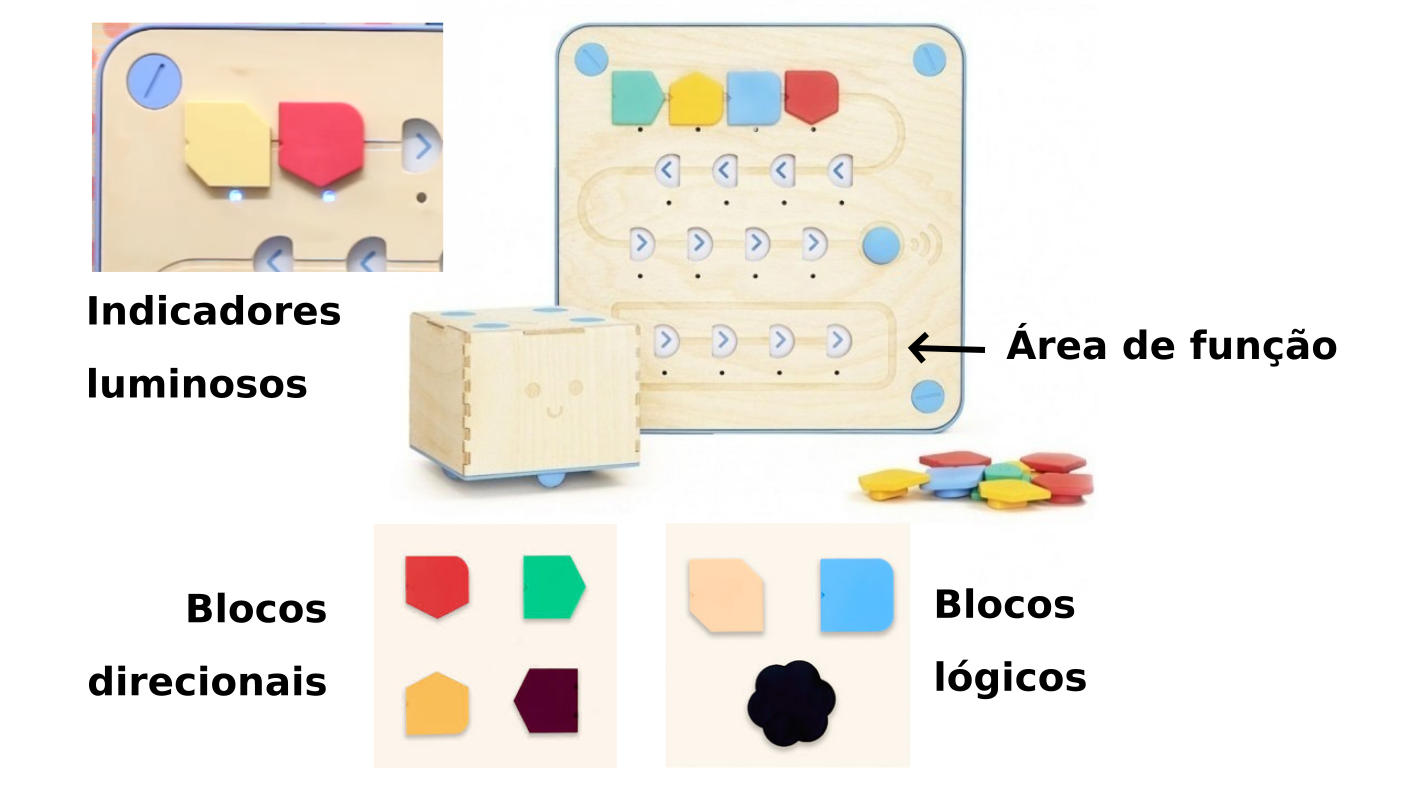
\includegraphics[width=.7\linewidth,fbox]{figs/cubetto_blocks.png}
    \caption{Cubetto: indicadores luminosos, área de função e blocos.}
    \label{fig:cubetto_features}
\end{figure}

O painel do Cubetto possui 16 reentrâncias para encaixe dos blocos, sendo 12 reservadas para o algoritmo principal e 4 dedicadas à área de função. Para cada reentrância há um indicador luminoso que acende quando o bloco é encaixado e pisca quando o bloco é executado. Essa indicação luminosa mostra a sequência de execução de cada bloco, o que é particularmente útil para os blocos de negação e de função. Como o bloco de negação tem sua ação associada ao bloco seguinte (inverte a ação do bloco seguinte), ambos piscam. O mesmo ocorre com o bloco de função, que pisca enquanto os blocos na área de função são executados.

Neste sentido, o design do Cubetto busca tornar visível tanto as instruções do algoritmo quanto destacar cada passo durante a execução. A estrutura é visível por meio dos blocos e do \textit{feedback} luminoso fornecido ao encaixar um bloco no painel. Já a execução é indicada por meio do piscar embaixo de cada bloco. Essa visibilidade facilita a interação das crianças e a formação do modelo mental sobre como as peças se relacionam e modificam o comportamento do brinquedo. Os movimentos lentos do brinquedo, associados a indicação de quais peças estão sendo executadas beneficiam o entendimento do algoritmo e facilitam a depuração. Essas característica fizeram o projeto receber diversos prêmios de design\footnote{
\begin{itemize}
    \item London Design Award (2016) - \url{https://drivenxdesign.com/LON16/project.asp?ID=15112}
    \item German Design Award (2017) - \url{https://www.german-design-award.com/en/the-winners/gallery/detail/9304-cubetto.html}
    \item RedDot Award (2016) - \url{https://www.red-dot.org/project/cubetto-26086}
\end{itemize}
}.

\subsection{Bee-Bot com mesa interativa}
\citeonline{beraza_soft_2010} criaram uma mesa interativa para ser utilizada com a Bee-Bot por crianças de 4-5 a 12-14 anos. Essa mesa tem superfície semitransparente, na qual um projetor cria mapas virtuais interativos, projetando-os por baixo. A imagem projetada muda de acordo com os movimentos da Bee-Bot e acompanha a manipulação de outros elementos tangíveis. Por exemplo, quando a Bee-Bot passa de um quadrado para outro do mapa projetado, este quadrado é destacado.

A projeção de elementos virtuais de acordo com os elementos tangíveis ocorre devido à marcas fiduciais da biblioteca reacTIVision coladas na parte inferior desses elementos. Como a superfície da mesa é semitransparente, uma câmera embaixo da mesa consegue captar as marcas fiduciais. As imagens captadas são analisadas por um software que controla as projeções.

Além da mesa, o trabalho propõe a criação de um software de apoio aos professores para que criem e configurem as atividades com o brinquedo programável. Esse software busca atender aos seguintes requisitos:

\begin{itemize}
    \item Ter tapetes ou cenários adaptados para cada atividade;
    \item Poder interromper uma atividade e continuar depois;
    \item Registrar o progresso das crianças em determinado problema e acompanhar sua evolução no tempo;
\end{itemize}

\begin{figure}[!h]
    \centering
    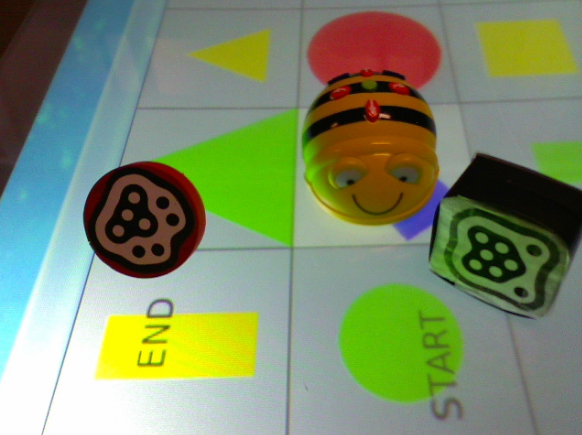
\includegraphics[width=.6\linewidth,fbox]{figs/beraza_bee_bot.png}
    \caption{Mesa interativa com a Bee-Bot.}
    \label{fig:beraza}
    \source{\citeonline{beraza_soft_2010}}
\end{figure}

Uma atividade de demonstração permite entender as potencialidades da tecnologia (\autoref{fig:beraza}). Nessa atividade, o usuário pode decidir o mapa a ser utilizado; decidir as posições de início e fim do trajeto a ser percorrido; e ver o trajeto percorrido com o número de passos executados. A visualização do trajeto percorrido permite à criança refletir sobre os comandos inseridos e depurar possíveis erros.

Nessa demonstração, cada quadrado do mapa contém uma forma geométrica de cor e tamanho variado. Isso possibilita que a criança exercite a classificação e abstração. A classificação seria a habilidade de identificar propriedades ou categorias, e relacionar essas categorias ou classes entre si. Nessa atividade, a criança classifica formas geométricas por propriedades como cor, formato e tamanho. Assim, a criança aprende a abstrair e observar apenas as propriedades relevantes para formar uma categoria. Esse mesmo tipo de tapete com formas geométricas é utilizado pelo brinquedo RoPE, porém em seu formato físico.

\subsection{ALERT}

O ALERT \cite{burleson_active_2018}, assim como os trabalhos anteriores, é uma interface de programação de brinquedos programáveis. O seu diferencial é que o robô interpreta os comandos à medida que ficam acessíveis no seu campo de visão. Cada robô possui uma câmera, que detecta novos comandos quando o robô se move. Por exemplo, se o robô anda para frente e capta o comando “vire 90º à direita”, ele interpreta e executa esta ação. Nisto percebe-se o princípio do feedback imediato defendido por \citeonline{norman_design_1988}. A execução do comando imediatamente ao ser detectado pelo brinquedo explicita a relação entre comando e resultado.

Para identificar os comandos captados o sistema interpreta marcas fiduciais da biblioteca reactTIVision, assim como o trabalho de \citeonline{beraza_soft_2010}. Essas marcas podem estar fixadas em folhas impressas distribuídas pelo chão, coladas em outros robôs ou também ser projetadas na superfície.

A vantagem em relação à inserção de comandos por meio de botões é a variedade de comandos possível de desenvolver sem a necessidade de um botão físico. Pode haver, por exemplo, uma marca representando o comando “vire 180º” ou "toque um som" sem necessidade de alterações de hardware. A \autoref{fig:alert} demonstra o uso do ALERT. As marcas fiduciais aparecem no cenário partindo de um projetor e representam, segundo o autor, comida e as bordas do cenário. O personagem da direita também tem marcas fiduciais e isso permite ao personagem da esquerda identificá-lo.

\begin{figure}[!h]
    \centering
    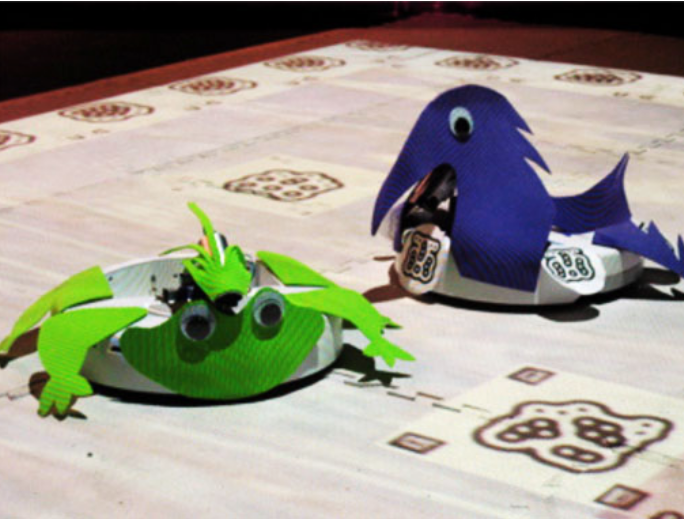
\includegraphics[width=.6\linewidth,fbox]{figs/alert.png}
    \caption{ALERT.}
    \label{fig:alert}
    \source{\citeonline{burleson_active_2018}}
\end{figure}

Com relação à depuração, a programação interativa se apresenta como um diferencial. A execução dos comandos à medida que o brinquedo os detecta, possibilita às crianças corrigirem o algoritmo durante a execução. Os autores exemplificam que se o brinquedo faz um movimento em U, quando o esperado era um giro à direita, as crianças podem adicionar novos comandos na frente dele. Deste modo a criança tem interação constante tanto com o robô quanto com o algoritmo, que se torna algo móvel.

\subsection{Análise Comparativa}

As seções anteriores apresentaram quatro trabalhos relacionados com programação de brinquedos programáveis.. Esta seção compara estes trabalhos quanto às seguintes características: idade do público-alvo, tipo de interface, e depuração (\autoref{quadro:comparision}). Por fim, os trabalhos são posicionados em relação à solução proposta.

Em relação ao público-alvo, o Robo-Blocks foca em crianças de 8 a 9 anos, pois a criança precisa entender basicamente o significado dos algarismos numéricos ao parametrizar o ângulo do giro do robô, e nesta idade as crianças normalmente aprenderam ler \cite{committee_on_the_prevention_of_reading_difficulties_in_young_children_preventing_1998}. Em contrapartida, o Cubetto, a Bee-Bot\footnote{Existem versões com texto nos botões \it{clear}, \it{go} e \it{pause}, mas os botões provocam sempre o mesmo comportamento. Mesmo que não saiba ler, a criança consegue mapear a ação do botão com sua funcionalidade.} e o ALERT não dependem diretamente de números, e por isso consegue atender um público a partir dos 4 ou 6 anos.

Com relação ao tipo de interface, todos os trabalhos utilizam interface tangível, mas seguindo diferentes abordagens. O Robo-Blocks tem blocos eletrônicos, que são encaixados entre si e possuem um display que mostra o tamanho do avanço ou giro. A programação do Cubetto também se dá por blocos tangíveis, porém sem visores e controles ajustáveis. Tudo o que a criança faz é encaixar os blocos em um painel. O ALERT tem blocos ainda mais simples. Foram usadas folhas de papel com as marcas fiduciais impressas, o que tende a ser mais barato e fácil de reproduzir. Por fim, a interface tangível da Bee-Bot não tem blocos, mas sim botões  \cite{yu_review_2019}. Apesar das diferentes abordagens, todos os trabalhos mencionam engajamento das crianças durante as interações, sejam elas com blocos eletrônicos, com as folhas de papel ou com os botões.

Por fim, em relação à depuração, o Robo-Blocks é a interface com maior foco em facilitar a atividade de encontrar erros em algoritmos. Isso se dá por duas características: marcadores físicos (bandeiras) para indicar possíveis erros, e a função de execução passo a passo.
No ALERT, os elementos de execução passo a passo são menos necessários. O brinquedo se move lentamente, e com isso há mais tempo para a criança olhar os comandos e comparar com os movimentos do robô. Além disso, o algoritmo pode ser alterado durante a execução. Se um comando desvia o brinquedo da rota, os passos subsequentes podem ser alterados para reajustá-la. A associação entre comando e ação também é mais óbvia no ALERT, pois o brinquedo precisa se aproximar do comando a ser executado. Quando um erro ocorre, fica claro qual foi o comando responsável. Quando os blocos eletrônicos ficam distântes do brinquedo esse mapeamento entre comando e ação é menos óbvio. Segundo  \citeonline{sipitakiat_robo-blocks_2012} as funções de depuração foram uma tentativa de resolver esse problema de mapeamento. A depuração no Cubetto é similar ao Robo-Blocks, pois o painel de programação fica distante do robô. Além disso, o Cubetto não tem execução passo a passo. Por fim, a interface de RA utilizada com a Bee-Bot  \cite{beraza_soft_2010} não tem visibilidade de código e nem funções de execução passo a passo, mas é similar ao trabalho aqui apresentado devido às tecnologias empregadas.

{{\renewcommand{\arraystretch}{1.5}
    \begin{quadro}[!h]
        \captionquadro{Análise comparativa.}
        \begin{tabularx}{\textwidth}{ @{} | p{.2\linewidth} | p{.1\linewidth} | X | X | @{} }
        \hline
        \textbf{Projeto ou ferramenta}  & \textbf{Idade do público-alvo}  & \textbf{Tipo de interface}       &\textbf{Depuração}                                          \\ \hline
        
        Robo-Blocks                     & 8 a 9 anos                      & Tangível com blocos eletrônicos  & Execução passo a passo, protractor e marcadores de erros   \\ \hline
        Cubetto                         & 4 a 8 anos                      & Tangível com painel eletrônico   & Destaca blocos em execução                                 \\ \hline
        Bee-Bot com mesa interativa     & 4-5 a 12-14 anos                & Tangível com botões              & -                                  \\ \hline
        ALERT                           & 6 anos                          & Tangível com projeção            & Permite alterar o comportamento do robô durante a execução \\ \hline
        RoPE AR                   & 4 a 6 anos                      & Tangível com projeção            & Destaca blocos em execução                                 \\ \hline
        \end{tabularx}
        \vspace{-10pt}
        \sourceauthor
        \label{quadro:comparision}
    \end{quadro}
}

Os trabalhos apresentados usam diferentes abordagens visando o mesmo objetivo: facilitar os primeiros contatos de crianças com algoritmos. Os quatro trabalhos aplicam interfaces tangíveis, mas de diferentes formas: há o uso de painel, blocos e botões. Assim como estes, o RoPE AR também usa interface tangível. A diferença está na união do tangível com a realidade aumentada. O trabalho de \citeonline{beraza_soft_2010} e o ALERT também aplicam RA, mas não há associação entre elementos os virtuais e os blocos que formam o algoritmo. Isso não significa uma desvantagem dos trabalhos citados, mas aponta uma lacuna de investigação a que este trabalho busca preencher.

Outro diferencial do RoPE AR é a tentativa de facilitar a instalação e o transporte. Isso é importante para produtos a serem usados em sala de aula. O trabalho de \citeonline{beraza_soft_2010} necessita de uma mesa com tampa semi transparente e de um notebook. O RoPE AR, por outro lado, utiliza apenas um suporte para o projetor, um projetor pequeno e um smartphone.
Por fim, um último diferencial é que no RoPE AR a projeção ocorre por cima, o que permite projetar não apenas figuras numa superfície inferior aos elementos tangíveis, mas também \it{sobre} eles.

\section{Revisão Sistemática: Pesquisas de IHC com crianças}
\label{sec_rsl}
Para compreender como são feitas as pesquisas sobre brinquedos programáveis com crianças, o método utilizado foi o de revisão sistemática \cite{kitchenham_guidelines_2007}. Esse método é um tipo de estudo que revisa estudos a respeito de uma pergunta de pesquisa, tópico ou fenômeno de interesse. No processo busca-se identificar, avaliar e interpretar as publicações relevantes para o tema em questão, e evitar o viés de quem produziu a pesquisa. Três questões exploratórias guiaram a busca:

\begin{itemize}
    \item QE1 - Quais tipos de interfaces são usadas em pesquisas sobre aprendizado de algoritmos na Educação Infantil?
    \item QE2 - Quais métodos e design de experimentos são utilizados?
    \item QE3 - O que as crianças aprendem ao interagir com brinquedos programáveis?
\end{itemize}

A seguinte busca foi adaptada para os artigos publicados nos anos de 2015 a 2020 nos repositórios ACM Digital Library, ERIC, IEEE Xplore e Science Direct:

\destaque{(crianças ou "jardim de infância") E (atividades OU "práticas pedagógicas") E (robótica ou "brinquedos programáveis") E (pensamento computacional)}.

\subsection{Resultados}

Sobre os resultados obtidos com as buscas nos repositórios, foram aplicados os critérios de inclusão e exclusão primeiramente sobre os resumos e depois sobre o texto completo (\autoref{quadro_criterios}). Após a aplicação dos critérios, restaram 7 artigos.

\begin{quadro}[!htbp]
\caption{Critérios de inclusão e exclusão.}
\label{quadro_criterios}
 \centering
 \begin{tabular}{|p{.45\textwidth}|p{.45\textwidth}|}
 \hline
 Critérios de inclusão & Critérios de exclusão \\
    \hline
    
    \begin{minipage}{.45\textwidth}
        1. Estudos primários indicando intervenção relacionada a ensino/aprendizado de algoritmos na Educação Infantil \\
        2. Estudos publicados entre 2015 e 2020 \\
        3. Estudos com crianças entre 3 e 6 anos \\
    \end{minipage}
    
    &
    
    \begin{minipage}{.45\textwidth}
    \vspace{.5cm}
        1. Artigos em línguas diferentes de inglês e português \\
        2. Título ou resumo mencionando nível diferente de Educação Infantil \\
        3. Foco em formar professores \\
        4. Menos de 5 páginas  \\
        5. Estudos secundários ou terciários \\
        6. Estudos focados em público-alvo diferente desta pesquisa \\
        7. Estudos duplicados \\
        8. Estudo que não aborda criação de algoritmos por crianças \\
        9. Estudo cujo texto completo não foi possível acessar \\
    \end{minipage}

 \\ \hline
 
 \end{tabular}
\end{quadro}

O critério de inclusão 3 (idade entre 3 a 6 anos) filtrou 82 trabalhos, pois grande parte dos estudos tem público-alvo maior de 6 anos. O segundo critério que filtrou mais artigos (CI1) aplicou-se a 30 artigos que não apresentaram nenhum tipo de intervenção com crianças, a fim de mensurar resultados como a qualidade de alguma ferramenta ou aprendizado de algoritmos. Outros 15 trabalhos focaram em públicos específicos que se diferenciam do público desta pesquisa, e portanto foram desconsiderados. O \autoref{quadroartigosrsl} apresenta os artigos que passaram no filtro.

\begin{table}[!htbp]
    \begin{center}
    \begin{footnotesize}
    \caption{Resultados da RSL}
    \label{rsl_table}

    \begin{tabular}{|c|c|c|c|c|c|c|c|c|c|c|} \hline
        Repositório             & Res. & CE1 & CE2 & CE3 & CE4 & CE5 & CE6 & CE7 & CE8 & CE9 \\ \hline
        ERIC                    &   4  &   3 &   2 &  2 &  2 &  2 & 2  &  2 &  2 &  2 \\ \hline
        ACM Digital Library     &  39  &  33 &  11 & 11 & 10 &  7 & 3  &  3 &  2 &  2 \\ \hline
        Science Direct          &   7  &   7 &   3 &  3 &  3 &  2 & 2  &  2 &  2 &  2 \\ \hline
        IEEE Xplore             & 114  &  91 &  36 & 32 & 32 & 21 & 13 & 11 & 11 &  1 \\ \hline
        Filtrados pelo critério & -    &  30 &  82 &  4 &  1 & 15 & 12 &  2 &  1 & 10 \\ \hline
        Artigos restantes       & 164  & 134 &  52 & 48 & 47 & 32 & 20 & 18 & 17 &  7 \\ \hline
    \end{tabular}
    
    \end{footnotesize}
    \end{center}
    \sourceauthor
\end{table}

\begin{landscape}
\linespread{1}
\begin{footnotesize}
\begin{quadro}
 \captionquadro{Artigos resultantes da RSL}
 \label{quadroartigosrsl}
\end{quadro}
\begin{longtable}{|p{6cm}|p{8cm}|p{8cm}|}
    \hline
    
    Publicação & Métodos utilizados / interfaces & Resultados / aprendizados \\ \hline
    
    \endhead
    
    \citeonline{repiso_robotics_2019} \newline
    \textit{Robotics to develop computational thinking in early Childhood Education} &
    
    Intervenção com a Bee-Bot® durante 7 encontros. Pesquisa quantitativa, quasi-experimental, com pré e pós teste. As crianças programaram usando botões e cartas. A avaliação utilizou desafios de programação com histórias lúdicas. As professoras e pesquisadores atribuíram notas de 0 a 5 conforme \citeonline{bers_computational_2014}. &
    
    A intervenção causou resultados positivos no grupo experimental nos aspectos de sequenciamento, correspondência ação-instrução e depuração. \\ \hline
    
    \citeonline{nam_connecting_2019}
    \textit{Connecting Plans to Action: The Effects of a Card-Coded Robotics Curriculum and Activities on Korean Kindergartners} &
    
    Intervenção utilizou a TurtleBot durante 8 encontros de 90 minutos com 53 crianças, uma vez por semana. As crianças planejaram o deslocamento desenhando e programaram usando cartões. Pesquisa quantitativa, quasi-experimental, com pré e pós teste. As professoras participaram da intervenção, auxiliando as crianças. &
    
    Apresentou resultados positivos nas habilidades de sequenciamento e resolução de problemas para o grupo experimental. \\ \hline
    
    \citeonline{di_lieto_educational_2017}
    \textit{
    Educational Robotics intervention on Executive Functions in preschool children: A pilot study
    } &
    
    Intervenção com a Bee-Bot® durante 6 semanas, duas vezes por semana, sendo 75 minutos por sessão. Divisão em grupos de 3 a 4 crianças, cada criança com um robô. Aumento gradual do tamanho do caminho a ser percorrido. Execução de testes de programação e psicológicos (memória, visão espacial e atenção). Uso de pré e pós teste. &
    
    Resultados indicaram aumento da capacidade de atenção e memória de trabalho. Melhoria na habilidade de programação das últimas 3 sessões comparadas às 3 primeiras. \\ \hline
    
    \citeonline{sheehan_parent-child_2019}
    \textit{Parent-child interaction and children's learning from a coding application} &
    
    Pesquisa quantitativa. Em dupla com seus pais, 31 crianças interagiram com o ScratchJr durante 10 minutos. Pesquisadores gravaram e transcreveram as conversas entre pais e filhos. Foram extraídas falas sobre linguagem espacial e perguntas. A linguagem foi relacionada com a produção e compreensão de comandos. &
    
    Os pais utilizaram mais termos de linguagem espacial e fizeram mais perguntas do que seus filhos, para auxiliá-los. O número de perguntas foi um preditor negativo da produção e compreensão de comandos. \\ \hline
    
    \citeonline{pila_learning_2019}
    \textit{Learning to code via tablet applications: An evaluation of Daisy the Dinosaur and Kodable as learning tools for young children} &
    
    Pesquisa qualitativa com pré e pós teste. 28 crianças de 4 a 6 anos usaram, durante uma semana, 2 aplicativos para ensino de programação (Kodable e Daisy the Dinossaur). A pesquisa captou o quanto as crianças gostaram de cada aplicativo e a influência do gênero no desempenho. Também foi avaliado o reconhecimento de comandos antes e após a intervenção, com notas de 0 a 5 conforme \citeonline{bers_computational_2014}. &
    
    Testes t identificaram um aumento significativo no reconhecimento dos comandos do aplicativo Daisy. Após uma semana foi possível identificar a compreensão de habilidades gerais de codificação. O “apelo” do aplicativo teve correlação com o aprendizado resultante, e o gênero não afetou o desempenho. \\ \hline
    
    \citeonline{burleson_active_2018}
    \textit{Active Learning Environments with Robotic Tangibles: Children's Physical and Virtual Spatial Programming Experiences} &
    
    Pesquisa qualitativa comparando o uso de duas ferramentas de programação espacial, sendo uma virtual e outra tangível (Robopad e ALERT). 9 crianças de 6 anos, divididas em 4 grupos, interagiram durante 5 dias (num calendário de 2 semanas) com ambas as ferramentas. &
    
    Usando o ALERT as crianças foram capazes de programar, colaborativamente, sequências para alterar o comportamento do robô. A ferramenta Robopad induziu mais a alterar/depurar o “programa” em tempo de execução.  \\ \hline
    
    \citeonline{heljakka_gamified_2019}
    \textit{Gamified Coding: Toy Robots and Playful Learning in Early Education} &
    
    Pesquisa qualitativa. Durante um período de 6 meses os pesquisadores disponibilizaram os brinquedos programáveis Dash e Botley a duas professoras e 21 crianças de 5 anos. As crianças brincaram livremente com os brinquedos e as professoras registraram o quão rápido as crianças aprenderam a programá-los. Os pesquisadores visitaram a sala de aula e entrevistaram crianças e professoras. &
    
    As crianças aprenderam a programar os brinquedos e também criaram brincadeiras, como criar um túnel com as pernas para o Dash passar e construir caminhos para o Botley percorrer. \\ \hline
    
    Esta pesquisa & Pesquisa mista. Coleta automática de interações. Uso do brinquedo RoPE com e sem realidade aumentada. & Pretende-se mensurar a colaboração, a depuração, e o número de erros ligados à lateralidade. \\ \hline
    
    \end{longtable}   
\end{footnotesize}

\end{landscape}

\subsection{QE1 - Quais tipos de interfaces são usadas em pesquisas sobre aprendizado de algoritmos na Educação Infantil? }

O tipo de interface mais citado nos resultados foram os brinquedos controlados por botões. A Bee-Bot apareceu em duas pesquisas, e outros brinquedos programados por botões foram a TurtleBot e o Botley. Aplicativos citados foram o ScratchJr, a interface do Dash, o Kodable, e \textit{Daisy the Dinossaur}. Outro tipo de interface citado é a espacial: \citeonline{burleson_active_2018} apresenta o ALERT e o Robopad, em que os agentes se movem no espaço e captam os comandos do ambiente.

Além das interfaces, outra variável a ser considerada são os tipos de atividades realizadas. Uma mesma interface, utilizada de modos diferentes, pode gerar diferentes aprendizados. A sequência de atividades do TangibleK Robotics Currículum, desenvolvida por \citeonline{bers_computational_2014} foi aplicada por \citeonline{repiso_robotics_2019} e por \citeonline{pila_learning_2019}. Dividida em 7 encontros, o primeiro dia de atividades iniciou com a exploração da interface da Bee-Bot, seguida (nos dias 2 e 3) da programação do brinquedo para se deslocar sobre tapetes. Nos dias 4 e 5 foram introduzidas cartas correspondentes às instruções, para serem sequenciadas e depois comparadas com os movimentos do brinquedo. Nos dias 6 e 7 foram mostradas sequências de comandos com erros, e as crianças exercitaram a depuração ao encontrar esses erros.

\citeonline{di_lieto_educational_2017} apresenta atividades de dificuldade incremental, em que as crianças precisavem programar a Bee-Bot para se deslocar sobre um tapete de formas cada vez mais complexas. \citeonline{heljakka_gamified_2019} não definiram nenhuma atividade específica para as crianças, apenas permitiram a exploração dos brinquedos Botley e Dash por 6 meses.

\subsection{QE2 - Quais métodos e design de experimentos são utilizados?}

O método mais utilizado foi a pesquisa quasi-experimental, com pré e pós teste. Das 7 pesquisas, 4 foram quantitativas, 2 qualitativas e uma mista. Além disso, \citeonline{nam_connecting_2019} e \citeonline{repiso_robotics_2019} utilizaram grupo de controle e experimental.

O tempo das intervenções variou consideravelmente. As pesquisas objetivando mensurar efeitos decorrentes das interações com os brinquedos foram mais longas, durando de 7 encontros a 6 meses. A pesquisa que buscou avaliar a usabilidade foi mais rápida, durando 10 minutos.

As amostras utilizadas foram de conveniência, com experimentos realizados nos ambientes escolares. O tamanho das amostras variou entre 9 e 31 crianças, que trabalharam em grupos em 6 das 7 pesquisas. As fontes de dados utilizadas foram vídeos, mapa de eventos, rubricas, transcrições, e entrevistas.

\subsection{QE3 - O que as crianças aprendem ao interagir com brinquedos programáveis?}

Os trabalhos citam principalmente o aprendizado de sequenciamento e de algoritmos em geral. \citeonline{pila_learning_2019}, após a interação de um conjunto de crianças durante 5 dias com os aplicativos Daisy e Kodable, perguntaram às crianças “O que é programar?”. A nota máxima foi dada a respostas que apresentavam a ideia de causa e efeito aplicável à tecnologia em geral, por exemplo “programar é colocar código em algo para que faça alguma ação”. Os resultados indicaram que as crianças não evoluíram na capacidade de expressar verbalmente seu entendimento de codificação.

Um outro aspecto da compreensão algorítmica avaliado por \citeonline{repiso_robotics_2019} e \citeonline{pila_learning_2019} é a compreensão dos símbolos da interface. \citeonline{repiso_robotics_2019} investigaram a compreensão sobre a correspondência entre ação e instrução, que significa mapear qual ação o robô executa em correspondência a um símbolo. A partir das rubricas os pesquisadores identificaram uma evolução significativa no grupo experimental. \citeonline{pila_learning_2019} mostrou quatro símbolos da interface do aplicativo Daisy para as crianças e solicitou que explicassem verbalmente o significado do símbolo. No pré-teste a média de acerto foi de 0.5 e no pós-teste esse valor subiu para 2.3.

\citeonline{nam_connecting_2019} avançaram nessa compreensão e utilizaram um instrumento para captar a compreensão de sequências. O instrumento utilizado solicita que crianças organizem 4 imagens que mostram eventos sequenciais, dada a imagem inicial. Os resultados apontaram evolução significativa na pontuação de sequenciamento para o grupo experimental.

\section{Mapeamento Industrial: Interfaces de Brinquedos Programáveis}
\label{secao_mapeamento_industrial}

O mapeamento industrial buscou encontrar o maior número possível de brinquedos programáveis que estão ou estiveram disponíveis para comercialização\footnote{O mapeamento fez parte de uma pesquisa voltada a brinquedos com características inteligentes, como IA e IoT. Nesta seção os dados serão avaliados com foco em realidade aumentada.}. A busca por estas fontes se justifica por abranger empresas e produtos que não estão diretamente ligados a publicações acadêmicas. Portanto, a pesquisa não utilizou bases científicas, mas sim plataformas de comércio eletrônico e buscadores. O mapeamento seguiu três etapas \cite{cooper_alice:_2000}:
\begin{enumerate}
    \item Definição das questões de pesquisa
    \item Planejamento do processo de busca
    \item Definição dos critérios para filtrar os resultados
\end{enumerate}

As próximas subseções detalham essas etapas da forma mais transparente possível.

\subsection{Questões de Pesquisa}

Três questões exploratórias guiaram o processo de busca:

\begin{enumerate}
    \item Quais são os tipos de interfaces mais frequentemente utilizados em brinquedos programáveis?
    \item Como a realidade aumentada é aplicada em brinquedos programáveis?
    \item Quais são os conceitos de algoritmos abordados?
\end{enumerate}

\subsection{Processo de Busca}
A segunda etapa define a \textit{string} de busca a ser aplicada em campos de pesquisa. O foco esteve em programação, resultando na seguinte \textit{string}:

\textit{ ((coding OR programmable) AND toys) }.

Seguindo a estratégia também apresentada no mapeamento feito por \citeonline{kitchenham_guidelines_2007}, uma exploração inicial indicou o uso das seguintes fontes de busca:

\begin{itemize}
    \item Plataforma de comércio eletrônico Amazon.com
    \item Postagens de blogs encontrados em pesquisas no Google e no DuckDuckGo
    \item Plataforma de financiamento coletivo Kickstarter.com
    \item Vídeos do Youtube
\end{itemize}

Além destas fontes, uma lista de páginas online selecionadas pelo orientador desta pesquisa durante estudos sobre o tema contribuiu como fonte de busca.

A string de busca foi aplicada nos sites que oferecem campos de pesquisa. Outra fonte de busca foram as categorizações de produtos existentes nos websites. O site kickstarter.com, por exemplo, tem uma área específica sobre projetos de robótica, enquanto a plataforma amazon.com possui uma categoria de produtos denominada \textit{coding toys}. Essas categorizações foram consultadas e os resultados adicionados aos resultados da busca textual. Por fim, a abrangência do mapeamento foi validada por meio da consulta de artigos de revisão a fim de encontrar brinquedos faltantes. Nessa etapa 5 brinquedos foram adicionados.

\subsection{Filtro}
Os critérios de inclusão foram três. Primeiramente, a presença de alguma forma de inserir comandos a serem executados pelo brinquedo. O segundo critério é a presença de algum componente tangível, ou seja, aplicativos sem interação com brinquedo físico foram descartados. O último critério é a presença de algum componente eletrônico, de forma que haja um processamento dos comandos programados para controlar sua execução. Esse critério eliminou os jogos de tabuleiro e livros de programação \cite{hamilton_emerging_2020}.

Após encontrar brinquedos adequados aos critérios de inclusão, a próxima etapa foi obter dados sobre as interfaces de programação. Para cada brinquedo foi executada uma pesquisa por vídeos demonstrando o uso do brinquedo. Outras fontes de dados foram as descrições presentes nas páginas de comércio eletrônico e páginas dos fabricantes.

\subsection{Resultados}
Um total de 86 brinquedos resultaram do processo de busca. Destes, 56 serviram como objeto de análise para responder às três perguntas de pesquisa. Os outros 30 brinquedos não foram analisados por terem sido adicionados à lista posteriormente ou por serem versões similares de algum dos brinquedos analisados. Os resultados estão disponíveis no endereço \url{https://bit.ly/35cUbZ1}. O \autoref{quadro:toys_reviewed} sumariza os brinquedos utilizados na análise.
\begin{landscape}
\linespread{1}
\begin{quadro}
 \captionquadro{Brinquedos resultantes do mapeamento industrial.}
 \label{quadro:toys_reviewed}
\end{quadro}
\begin{small}
\begin{longtable}{|p{4.5cm} p{4.5cm} r| p{4.5cm} p{4.5cm} r|}
    \hline
    Nome & Fabricante & Ano & Nome & Fabricante & Ano \\ \hline
    Big Trak / Big Track Junior & Milton Bradley & 1979 &
    Sphero SPRK+ & Sphero & 2016 \\ \hline
    Topobo & MIT Tangible Media Group & 2003 &
    Go Robot Mouse & Learning Resources & 2016 \\ \hline
    Finch & BirdBrain Technologies & 2010 &
    Coji & WowWee & 2016 \\ \hline
    Bee-Bot & TTS Group & 2011 &
    KUMIITA & ICON Corp & 2016 \\ \hline
    KIBO & Kinderlab Robotics & 2012 &
    RoPE & SmartFun Brasil & 2017 \\ \hline
    Dr. Wagon & Stanford & 2012 &
    Harry Potter Coding Kit & KANO & 2017 \\ \hline
    Ollie & Sphero & 2012 &
    Meccano-Erector Meccanoid & Spin Master & 2017 \\ \hline
    RoboTami Creative Robot Kit & Robotron & 2012 &
    Lego Boost & Lego & 2017 \\ \hline
    Lego Mindistorms EV3 & Lego & 2013 &
    Anki Cozmo & Digital Dreams & 2017 \\ \hline
    Romo & Romotive & 2013 &
    Sam Curious Cars Kit & Sam Labs & 2017 \\ \hline
    Pro-Bot & TTS Group & 2014 &
    Airblock & Makeblock & 2017 \\ \hline
    Dot & MakeWonder & 2014 &
    Augie & Pai Technology & 2017 \\ \hline
    Dash & MakeWonder & 2014 &
    Minion Mip & WowWee & 2017 \\ \hline
    Edison & Edison & 2014 &
    Miko 2 & Miko & 2018 \\ \hline
    Ozobot & Ozobot & 2014 &
    Kids First Coding e Robotics & GIGO & 2018 \\ \hline
    TinkerBots & TinkerBots & 2014 &
    Botley & Learning Resources & 2018 \\ \hline
    TiddlyBot & Agilic & 2014 &
    Q-Scout & RoboBloq & 2018 \\ \hline
    Guimo & Guimo Toys & 2015 &
    InO-Bot & TTS Group & 2018 \\ \hline
    BlueBot & TTS Group & 2015 &
    Codey Rocky & Makeblock & 2018 \\ \hline
    Osmo Coding & Tangible Play Inc & 2015 &
    Aibo - ERS-1000 & Sony & 2018 \\ \hline
    Cubetto & PrimoToys & 2015 &
    Root & iRobot & 2018 \\ \hline
    Cue & MakeWonder & 2015 &
    Rugged Robot & TTS Group & 2019 \\ \hline
    Vortex & DFRobots & 2015 &
    Aukfa / JDBaby / HBuds & Aukfa & 2019 \\ \hline
    mBot & Makeblock & 2015 &
    Qobo & Robobloq & 2019 \\ \hline
    Robotiky & Robotiky & 2015 &
    mTity & Makeblock & 2019 \\ \hline
    SmartiBot & The Crafty Robot & 2015 &
    Botzees & Pai Technology & 2019 \\ \hline
    Robo Wunderkind & Robo Wunderkind & 2015 &
    Mojobot & Project Lab & 2019 \\ \hline
    Code a Pillar / Codipédia & Fisher Price - Mattel & 2016 &
    Mochi & Mochi & 2019 \\ \hline
\end{longtable}
\end{small}
\end{landscape}

Quanto ao ano de lançamento, mais de 80\% dos brinquedos foram lançados depois de 2014, o que corresponde ao crescimento do interesse pelo assunto \acl{PC}. A \autoref{toys_year} demonstra o número de brinquedos lançados por ano, e, comparado com a \autoref{pc_interest}, percebe-se uma semelhança no crescimento e no período de aumento. Isso sugere que os brinquedos estão sendo lançados comercialmente em resposta à uma demanda no campo educacional.

\begin{figure}[!htbp]
    \centering
    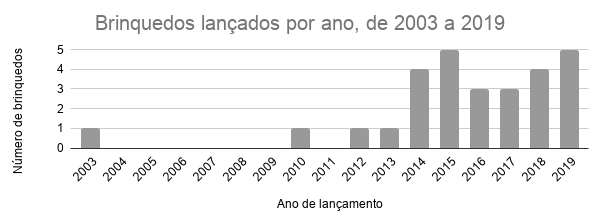
\includegraphics[width=.8\linewidth,fbox]{figs/brinquedos_ano.png}
    \caption{Brinquedos lançados por ano entre 2003 e 2019.}
    \label{toys_year}
    \sourceauthor
\end{figure}

\begin{figure}[!htbp]
    \centering
    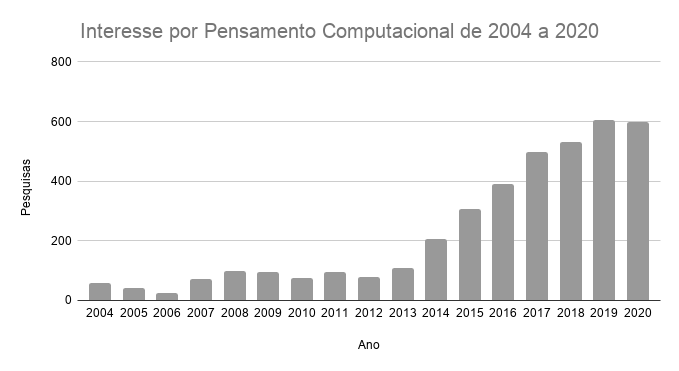
\includegraphics[width=.8\linewidth,fbox]{figs/pc_interest.png}
    \caption{Interesse pelo tema \acl{PC}, segundo o Google Trends.}
    \label{pc_interest}
    \sourceauthor
\end{figure}

\subsection{QE1 - Quais são os tipos de interfaces mais frequentemente utilizados em brinquedos programáveis?}

A resposta à pergunta \textit{QE1 - Quais são os tipos de interfaces mais frequentemente utilizados em brinquedos programáveis?} depende da perspectiva de análise dessas interfaces. Uma pesquisa pode observar os materiais utilizados, enquanto outra observar as cores e formas. O método utilizado para definir essa perspectiva foi o de Kawakita Jiro \citeonline{scupin_kj_1997}. Esse método busca organizar imagens em grupos em três fases: captura, agrupamento e categorização. Ao final é formado um diagrama de afinidades (\autoref{kj}).

\begin{figure}[!htbp]
    \centering
    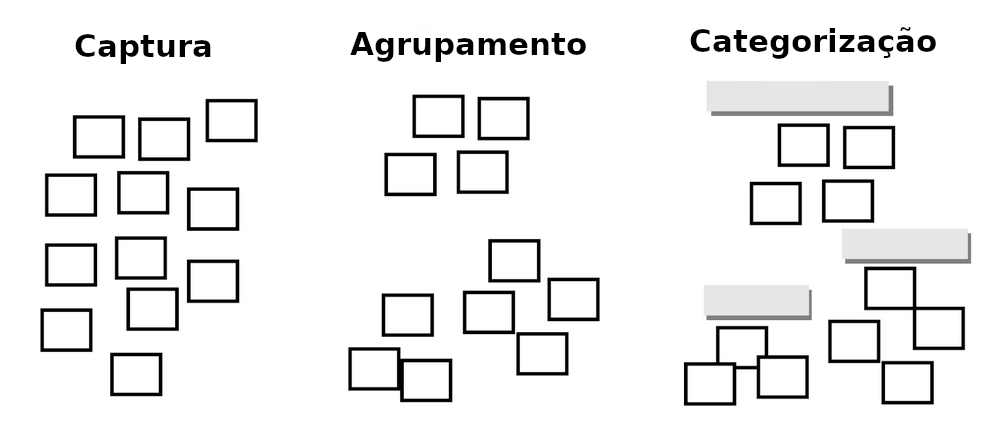
\includegraphics[width=.6\linewidth,fbox]{figs/kj.png}
    \caption{Método Kawakita Jiro.}
    \label{kj}
    \sourceauthor
\end{figure}
Na fase de captura, foram produzidos recortes de imagens focando nas interfaces dos brinquedos de programar. Essas imagens foram obtidas ao parar vídeos de demonstração dos brinquedos. Após a captura, imagens foram distribuídas em um software online e agrupadas por dois pesquisadores. Possíveis divergências, por exemplo, se blocos com texto e ícones pertencem a uma mesma categoria, foram discutidas e sanadas (\autoref{kj_run}).

\begin{figure}
    \centering
    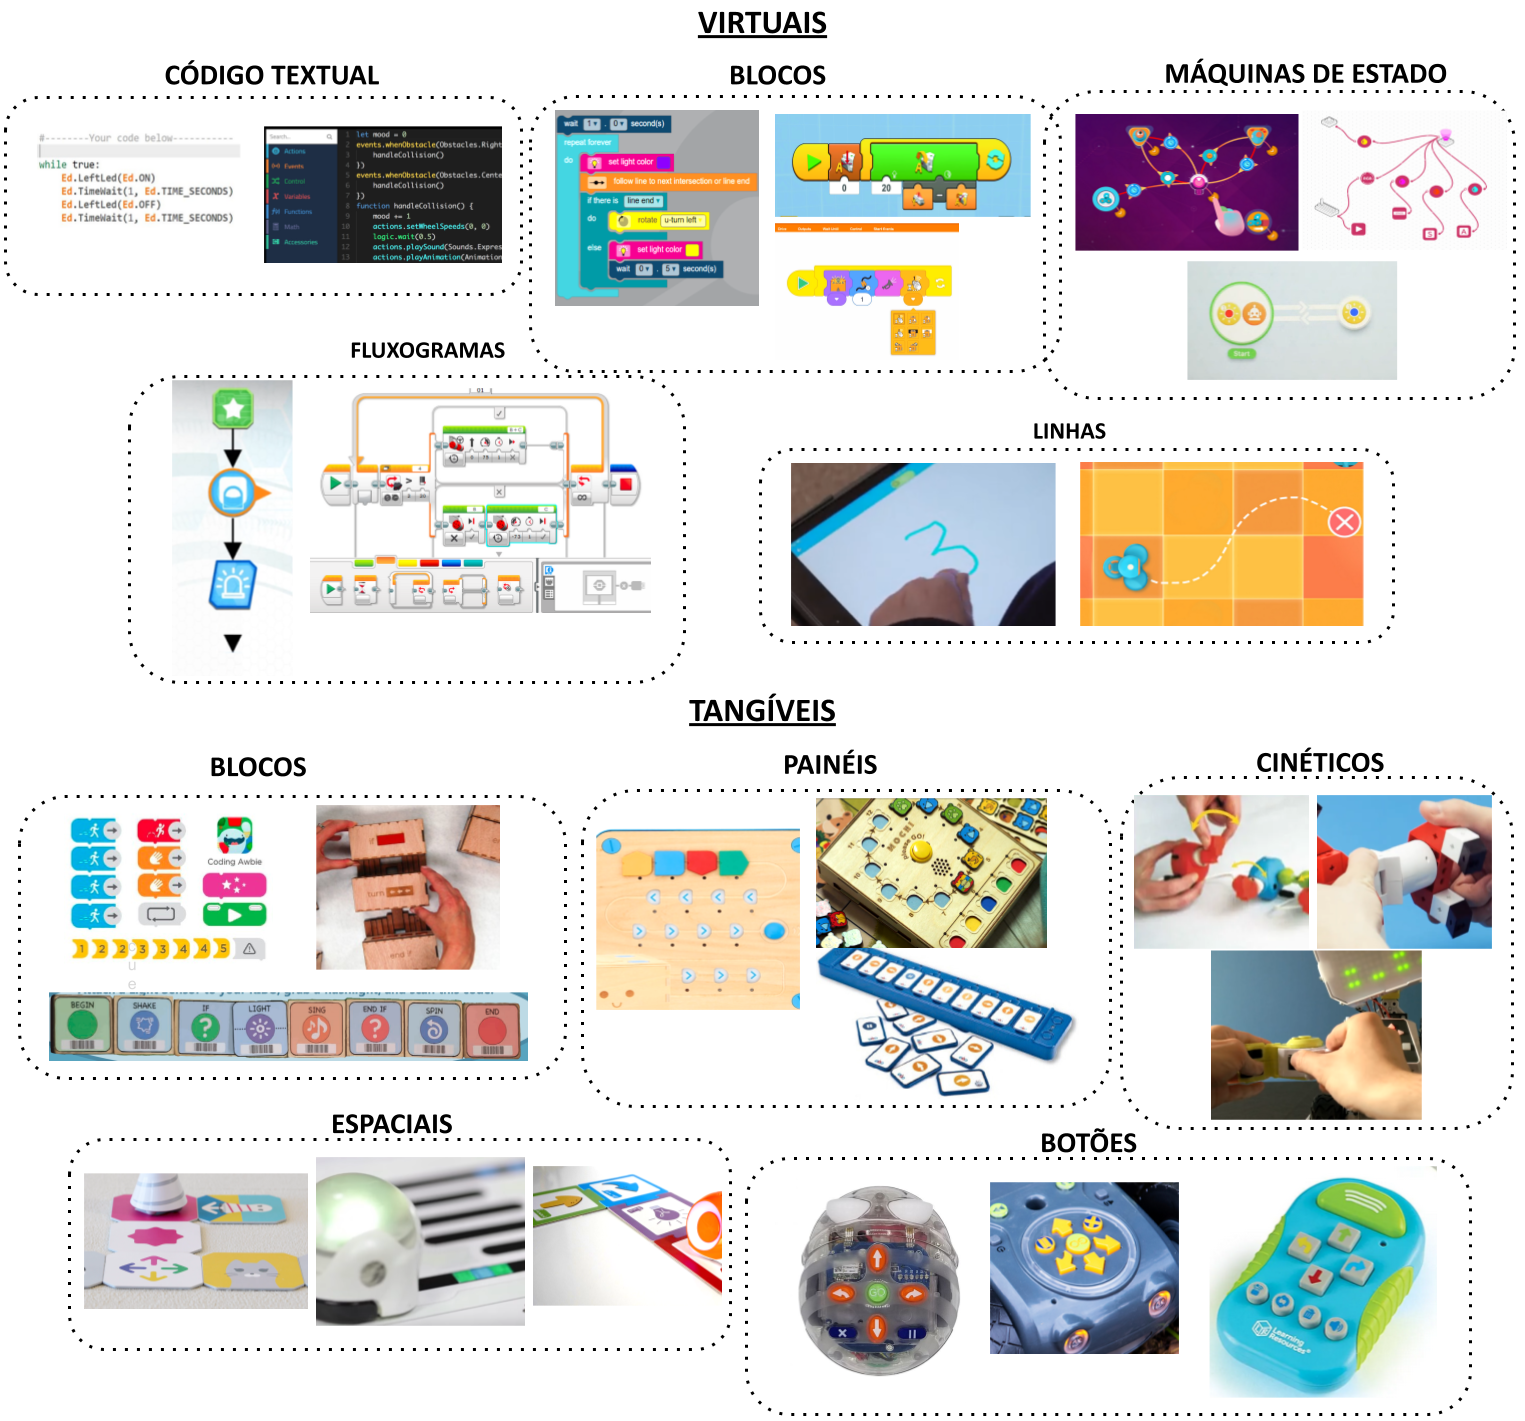
\includegraphics[width=1\linewidth,fbox]{figs/toys_interfaces.png}
    \caption{Agrupamento das interfaces.}
    \label{kj_run}
\end{figure}

O processo resultou em 2 categorias, cada uma com 5 subcategorias. A primeira categoria são as interfaces virtuais, onde há presença de uma tela bidimensional onde os comandos aparecem. A segunda categoria são as interfaces tangíveis, em que a interação ocorre com objetos físicos, como blocos de encaixar ou botões acoplados no brinquedo.

As subcategorias elencadas das interfaces virtuais foram:
\begin{description}
    \item[Código textual: ] Interfaces que usam código digitado em teclados, como as linguagens de propósito geral.
    \item[Blocos virtuais: ] Peças de quebra-cabeça que são conectadas e representam estruturas de programação.
    \item[Máquinas de estado: ] Formas geométricas conectadas por linhas, em que cada forma agrupa ações do brinquedo. As linhas representam eventos que provocam a transição entre os estados.
    \item[Linhas: ] Uma linha é desenhada na tela do dispositivo e o brinquedo se move conforme o seu formato.
    \item[Fluxogramas: ] Formas geométricas conectadas por linhas. Cada forma representa uma ação ou uma decisão.
\end{description}

As subcategorias de interface tangível são semelhantes.

\begin{description}
    \item[Blocos físicos: ] Blocos físicos que podem ser interconectados e não precisam ser fixados a um painel. Exemplos: Code a Pillar e KIBO.
    \item[Painéis: ] Placas de madeira ou de plástico com furos para encaixe de blocos de programação. Exemplos: Cubetto e Mojobot.
    \item[Cinéticos: ] Brinquedos que repetem os movimentos feitos em partes do corpo do brinquedo. Exemplo: Topobo.
    \item[Espacial: ] Brinquedo lê comandos do ambiente usando sensores.
    \item[Botões: ] Botões físicos acoplados ao corpo do brinquedo ou em um controle remoto.
\end{description}

Considerando essa taxonomia, o tipo mais comum de interface de brinquedos programáveis são os blocos virtuais, usados por 30 brinquedos. O segundo tipo mais usado são os botões. Outra tendência observada é o uso de mais de um tipo de interface pelo mesmo brinquedo, a fim de atender um público mais amplo quanto à faixa etária. A \autoref{toys_per_interface_type} descreve o uso de cada um dos tipos de interface.

\begin{figure}[!htbp]
    \centering
    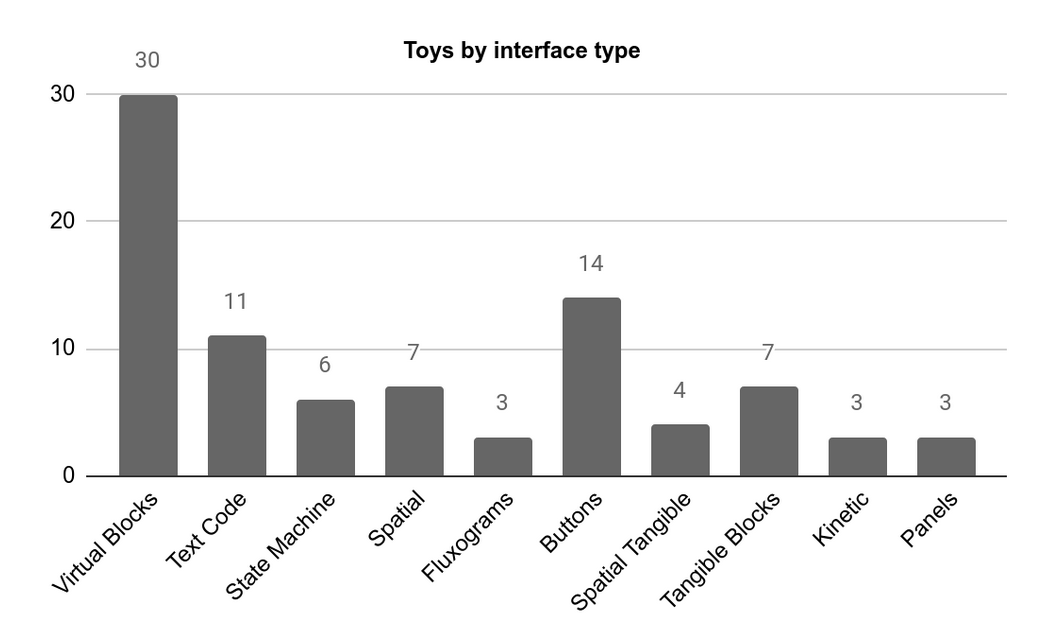
\includegraphics[width=.6\linewidth,fbox]{figs/toys_per_interface_type.png}
    \caption{Brinquedos por tipo de interface.}
    \label{toys_per_interface_type}
    \sourceauthor
\end{figure}

\subsection{QE2 - Como a realidade aumentada é aplicada em brinquedos programáveis?}
A \ac{RA}, no sentido de combinar objetos virtuais e físicos, é pouco usada em brinquedos programáveis. Dos 56 brinquedos encontrados, apenas 2 seguem essa abordagem: o Botzees e o Augie. Ambos os brinquedos são da empresa \textit{Pai Technology}, a qual apresenta o uso de \ac{RA} como um diferencial da marca.

O tipo de RA utilizado é o \textit{window-on-the-world}, ou seja, um \textit{tablet} ou \textit{smartphone} captura a imagem do brinquedo e associa objetos virtuais à imagem real na tela. No caso do Augie, o brinquedo é captado pela câmera e, ao ter sua posição identificada, os personagens aparecem na tela simulando uma batalha com o brinquedo físico. A RA também é usada para mostrar um mapa virtual na tela do \textit{tablet}, e o brinquedo físico percorre esse mapa (\autoref{augie_ar_programming}). O mesmo princípio se aplica ao Botzees. O \textit{smartphone} capta a imagem do brinquedo e mostra a imagem deste ao lado dos blocos virtuais (\autoref{botzees_ar_programming}).

Uma vantagem possível dessa abordagem é a proximidade com que o brinquedo físico e os blocos virtuais aparecem na tela. Isso diminui a necessidade de olhar para dois lugares ao mesmo tempo, ou seja, olhar para a tela do aplicativo e para o ambiente real. Porém não foram encontrados estudos que evidenciem benefícios deste tipo de interface para o aprendizado de programação por crianças.

\begin{figure}[!htbp]
    \centering
    \begin{subfigure}{.44\textwidth}
        \centering
        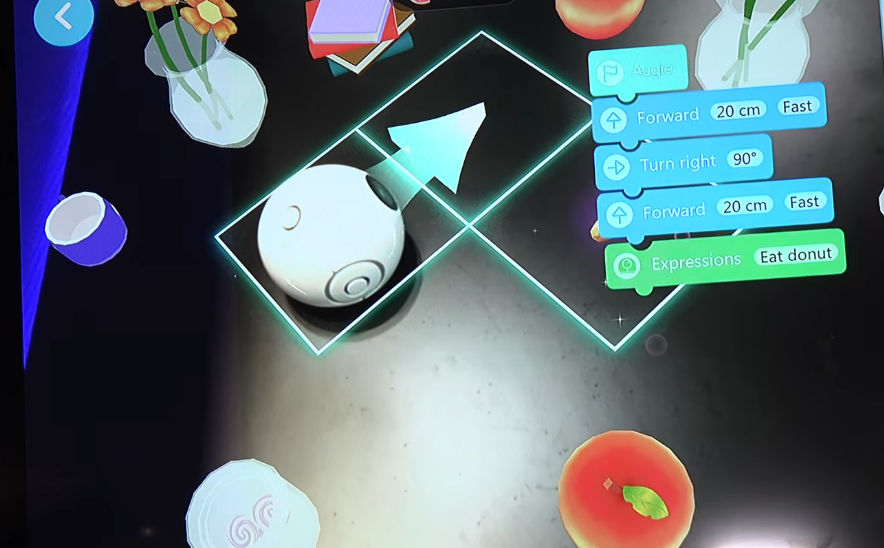
\includegraphics[width=.9\linewidth,fbox]{figs/augie_ar_programming_2.png}
        \caption{Programação do Augie com RA}
        \label{augie_ar_programming}
    \end{subfigure}%
    \begin{subfigure}{.55\textwidth}
        \centering
        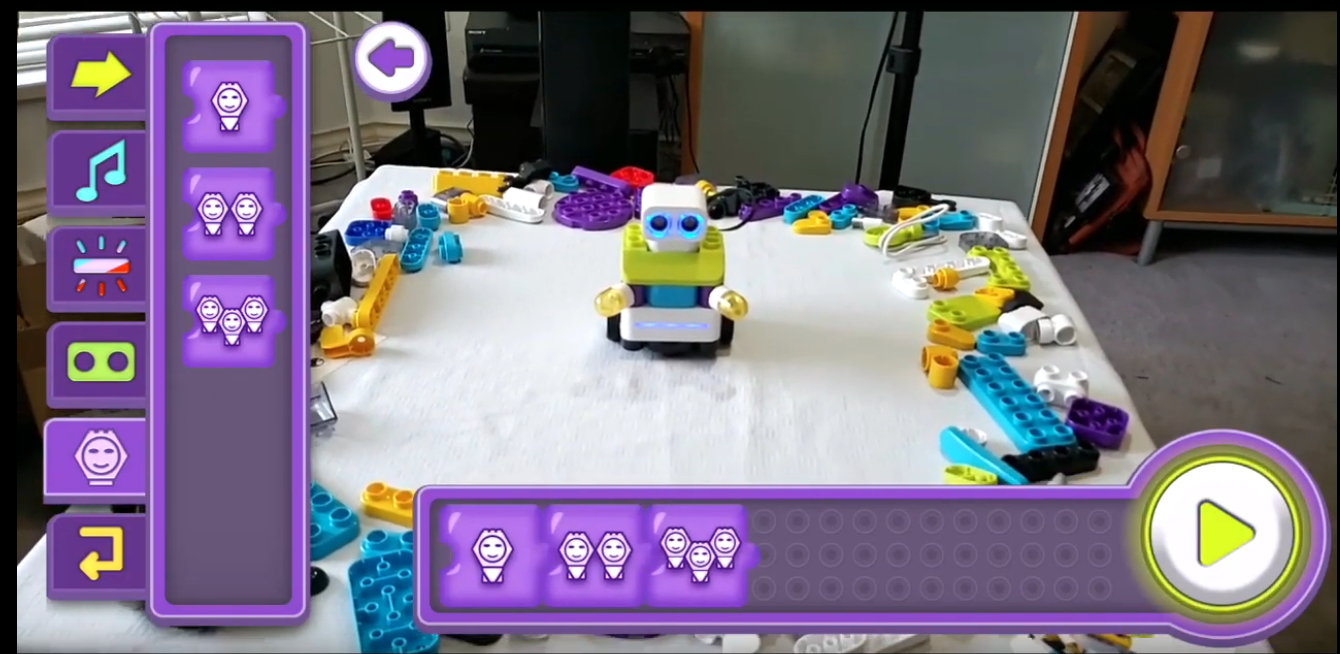
\includegraphics[width=.9\linewidth,fbox]{figs/botzees.png}
        \caption{Programação do Botzees com RA}
        \label{botzees_ar_programming}
    \end{subfigure}
    \caption{Usos de RA com brinquedos programáveis.}
    \label{ar_programming}
\end{figure}

\subsection{QE3 - Quais são os conceitos de algoritmos abordados nas interfaces de brinquedos programáveis?}

A abrangência de conceitos de algoritmos abordados por brinquedos programáveis foi analisada nos seguintes conceitos: variáveis, estruturas de repetição, condicionais, listas, recursividade, paralelismo, sequenciamento, funções, parâmetros e eventos. Aspectos como tipos de dados, constantes, orientação a objetos não foram abordados pois são abstraídos na maioria das interfaces.

\begin{figure}[!htbp]
    \centering
    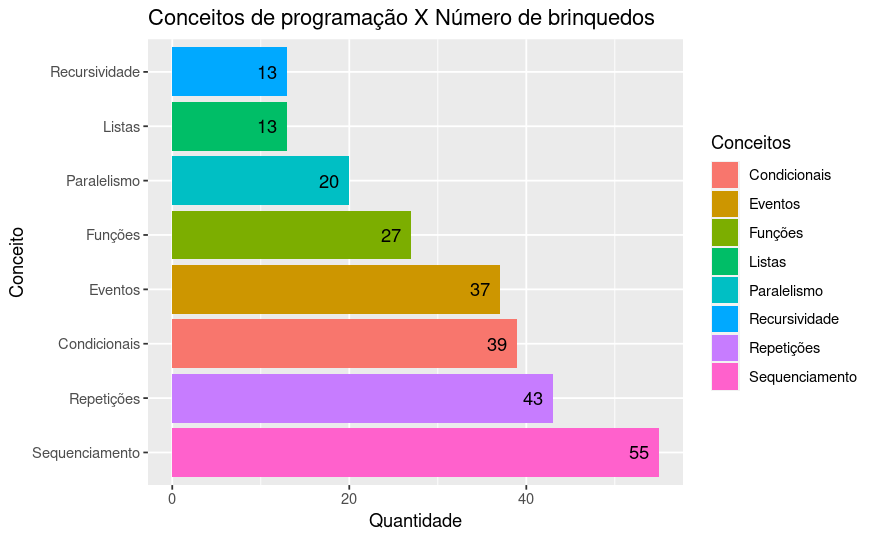
\includegraphics[width=.7\linewidth,fbox]{figs/conceitos_brinquedos.png}
    \caption{Conceitos de programação abordados por brinquedos programáveis.}
    \label{fig:toys_concepts}
    \sourceauthor
\end{figure}

A \autoref{fig:toys_concepts} apresenta o resultado da análise. Como o esperado, o sequenciamento é o conceito mais abordado: criar sequências de comandos a serem executados é intrínseco dos brinquedos programáveis. O segundo conceito mais abordado são repetições, por 76\% dos brinquedos. As estruturas de repetição são normalmente suportadas em interfaces virtuais de programação em blocos.

Outros dois conceitos interligados são condicionais e eventos. 66\% dos brinquedos disparam algum tipo de evento captado por sensores de luminosidade, proximidade, sons, etc. Esses eventos são usados em condicionais para ações do tipo "se obstáculo à frente", "se luminosidade maior que", entre outros.

Conceitos mais avançados, como paralelismo, recursividade e vetores são suportados pelos brinquedos que tem interfaces de código textual, com suporte a linguagens de propósito geral. Recursividade e vetores são conceitos suportados por 23\% dos brinquedos.

\section{Considerações}

Por fim, esse capítulo ressalta três aspectos. (i) O mapeamento industrial não apontou uso de realidade aumentada projetiva com brinquedos programáveis. Entretanto (ii) os trabalhos relacionados demonstram que usar projeção em interfaces de programação é viável e abre novas possibilidades de interação, como a programação espacial descrita por \citeonline{burleson_active_2018}. Além disso, o mapeamento indicou (iii) uso de interfaces tangíveis por 55\% dos brinquedos. A proposta apresentada no \autoref{c_desenvolvimento} considera esses três aspectos e busca representar um tipo inovador de interação, ou, ao menos, contribuir com pesquisas que indiquem a adequação da realidade aumentada projetiva aplicada à interfaces de brinquedos programáveis.
